\documentclass[c]{beamer}  % [t], [c], или [b] --- вертикальное выравнивание на слайдах (верх, центр, низ)
%\documentclass[handout]{beamer} % Раздаточный материал (на слайдах всё сразу)
%\documentclass[aspectratio=169]{beamer} % Соотношение сторон

\usetheme{Berkeley} % Тема оформления
%\usetheme{Berlin}
%\usetheme{Szeged}

\usecolortheme{seahorse} % Цветовая схема
%\useinnertheme{circles}
%\useinnertheme{rectangles}

%\usetheme{HSE}

%%% Работа с русским языком
\usepackage{cmap}					% поиск в PDF
\usepackage{mathtext} 				% русские буквы в формулах
\usepackage[T2A]{fontenc}			% кодировка
\usepackage[utf8]{inputenc}			% кодировка исходного текста
\usepackage[english,russian]{babel}	% локализация и переносы

%% Beamer по-русски
\newtheorem{rtheorem}{Теорема}
\newtheorem{rproof}{Доказательство}
\newtheorem{rexample}{Пример}

\usepackage{array}

%%% Дополнительная работа с математикой
\usepackage{amsmath,amsfonts,amssymb,amsthm,mathtools} % AMS
\usepackage{icomma} % "Умная" запятая: $0,2$ --- число, $0, 2$ --- перечисление
%\usepackage{multimedia}
%\usepackage{media9}

%% Номера формул
%\mathtoolsset{showonlyrefs=true} % Показывать номера только у тех формул, на которые есть \eqref{} в тексте.
%\usepackage{leqno} % Нумерация формул слева

%% Свои команды
\DeclareMathOperator{\sgn}{\mathop{sgn}}

%% Перенос знаков в формулах (по Львовскому)
\newcommand*{\hm}[1]{#1\nobreak\discretionary{}
{\hbox{$\mathsurround=0pt #1$}}{}}

%%% Работа с картинками
\usepackage{graphicx}  % Для вставки рисунков
\graphicspath{{pictures/}}  % папки с картинками
\setlength\fboxsep{3pt} % Отступ рамки \fbox{} от рисунка
\setlength\fboxrule{1pt} % Толщина линий рамки \fbox{}
\usepackage{wrapfig} % Обтекание рисунков текстом

%%% Работа с таблицами
\usepackage{array,tabularx,tabulary,booktabs} % Дополнительная работа с таблицами
\usepackage{longtable}  % Длинные таблицы
\usepackage{multirow} % Слияние строк в таблице

%%% Программирование
\usepackage{etoolbox} % логические операторы

%%% Другие пакеты
\usepackage{lastpage} % Узнать, сколько всего страниц в документе.
\usepackage{soul} % Модификаторы начертания
\usepackage{csquotes} % Еще инструменты для ссылок
%\usepackage[style=authoryear,maxcitenames=2,backend=biber,sorting=nty]{biblatex}
\usepackage{multicol} % Несколько колонок

%%% Картинки
\usepackage{tikz} % Работа с графикой
\usepackage{pgfplots}
\usepackage{pgfplotstable}

\title{Кусовая работа}
\subtitle{Численное моделирование динамики частиц дроби в рудоразмольной мельнице методом дискретных элементов}
\author{Катнов Артем}
\date{\today}
\institute[Факультет робототехники и комплексной автоматизации]{Московский государственный технический университет им. Н.Э.Баумана}

\usepackage{movie15}
\usepackage{hyperref}

\begin{document}

\begin{frame}
\maketitle
\end{frame}


\begin{frame}
\tableofcontents
\end{frame}

\section{Метод дискретных элементов}

\begin{frame}
\frametitle{\insertsection} 
\framesubtitle{\insertsubsection}

\begin{figure}[h!]
	\centering
	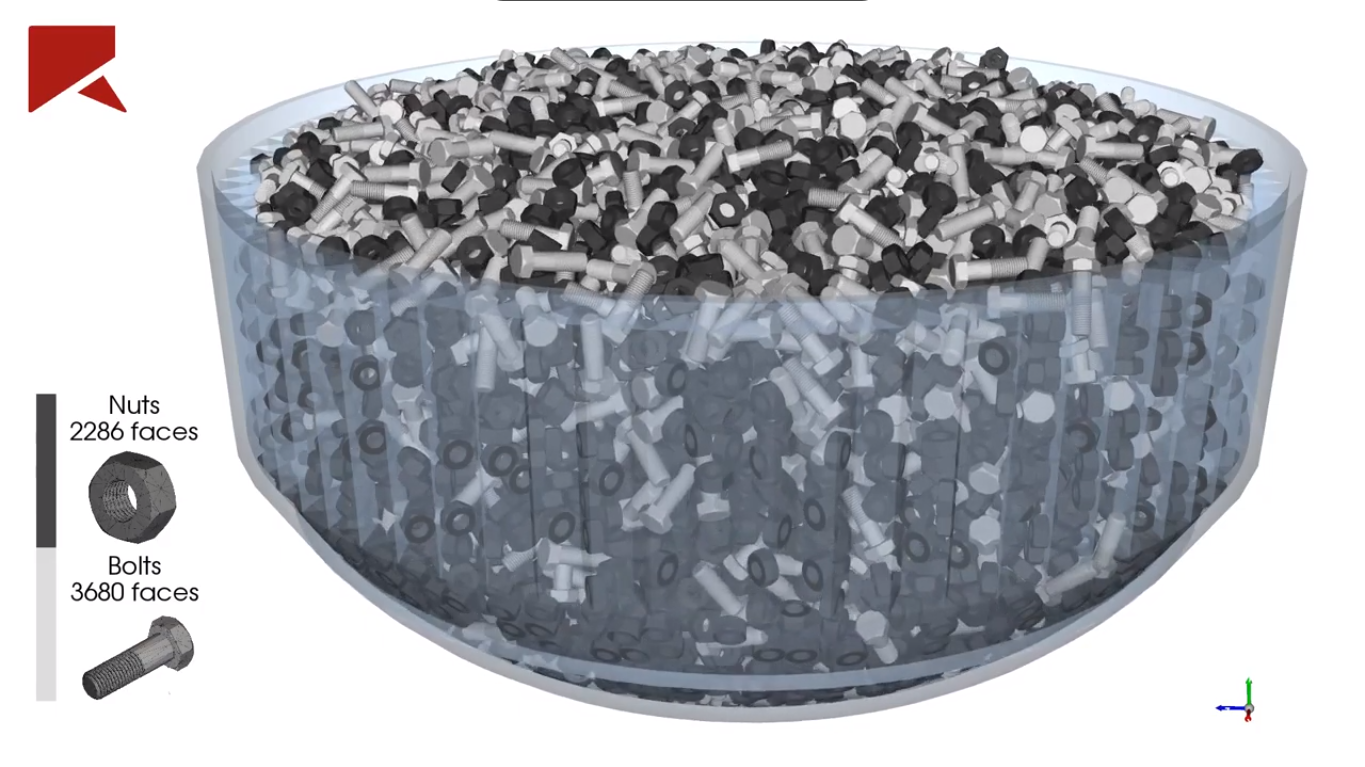
\includegraphics[width=0.4\textwidth]{sreda}
	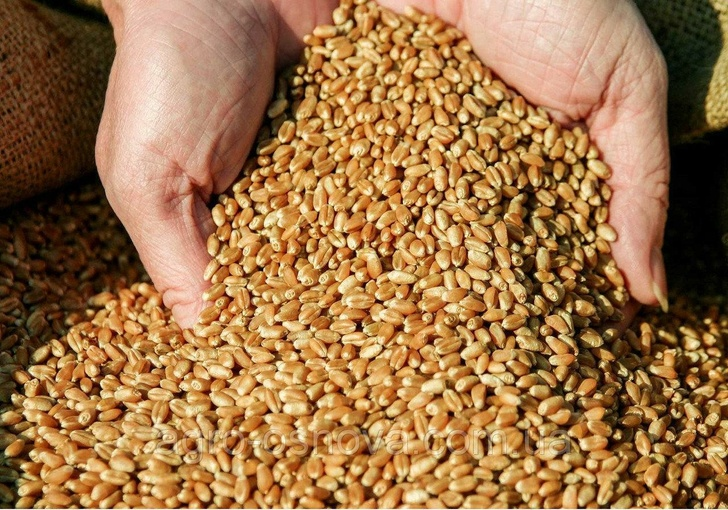
\includegraphics[width=0.4\textwidth]{sreda2}
	\caption{Демонстрация сыпучей среды}
\end{figure} 

Cundall P. A. A computer model for simulating progressive, large-scale movement in blocky rock system //Proceedings of the International Symposium on Rock Mechanics, 1971. – 1971.

\end{frame}

\begin{frame}
\frametitle{Цель работы} 
\framesubtitle{Шаровая мельница}

Цель работы: исследование динамики системы частиц дроби во вращающемся барабане рудоразмольной мельницы.

\begin{figure}[h!]
	\centering
	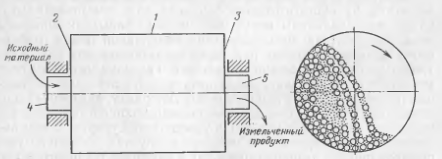
\includegraphics[width=0.7\textwidth]{baraban_shema}
	\caption{Схематическое изображение шаровой мельницы}
\end{figure}

 
\end{frame}






\begin{frame}
\frametitle{\insertsection} 
\framesubtitle{Алгоритм метода}

\begin{figure}[h!]
	\centering
	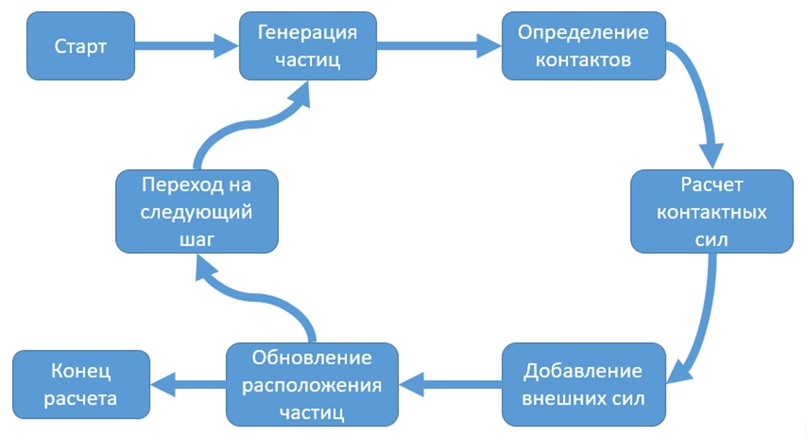
\includegraphics[width=0.9\textwidth]{algorithm}
	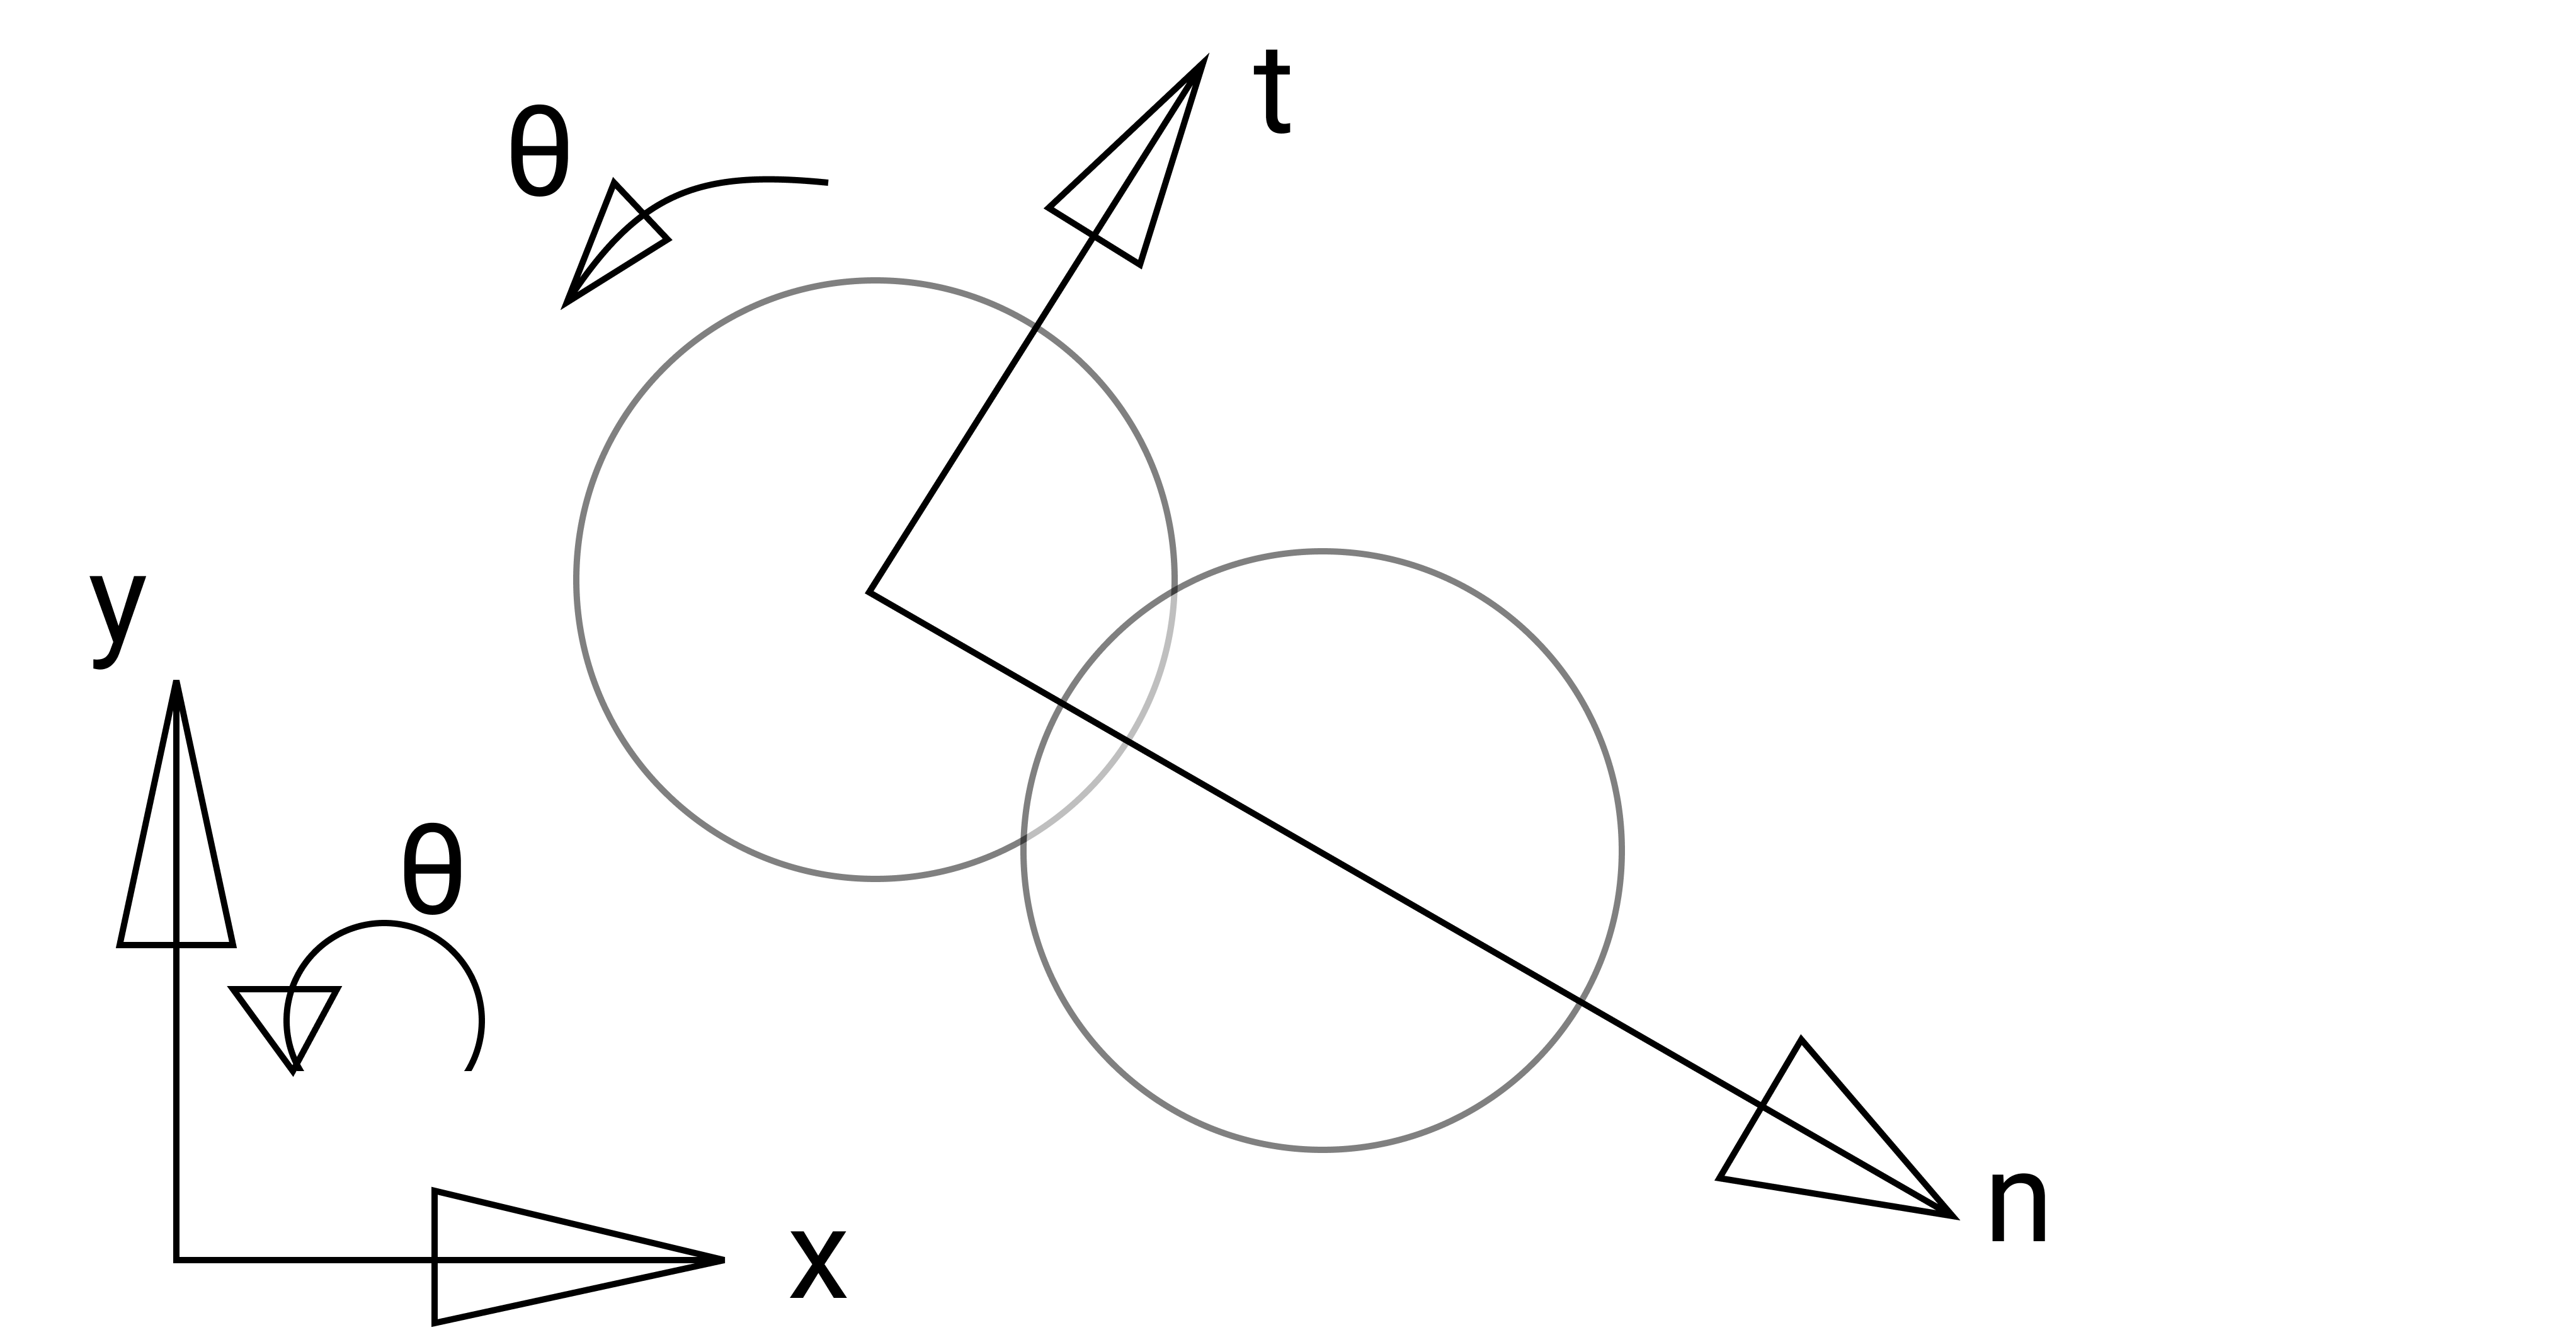
\includegraphics[width=0.5\textwidth]{local}
\end{figure} 
\end{frame}


\section{Описание модели}

\subsection{Контактные силы}




\begin{frame}
\frametitle{\insertsection} 
\framesubtitle{\insertsubsection}
Syed Z., Tekeste M., White D. A coupled sliding and rolling friction model for DEM calibration //Journal of Terramechanics. – 2017. – Т. 72. – С. 9-20.
\begin{figure}[h!]
	\centering
	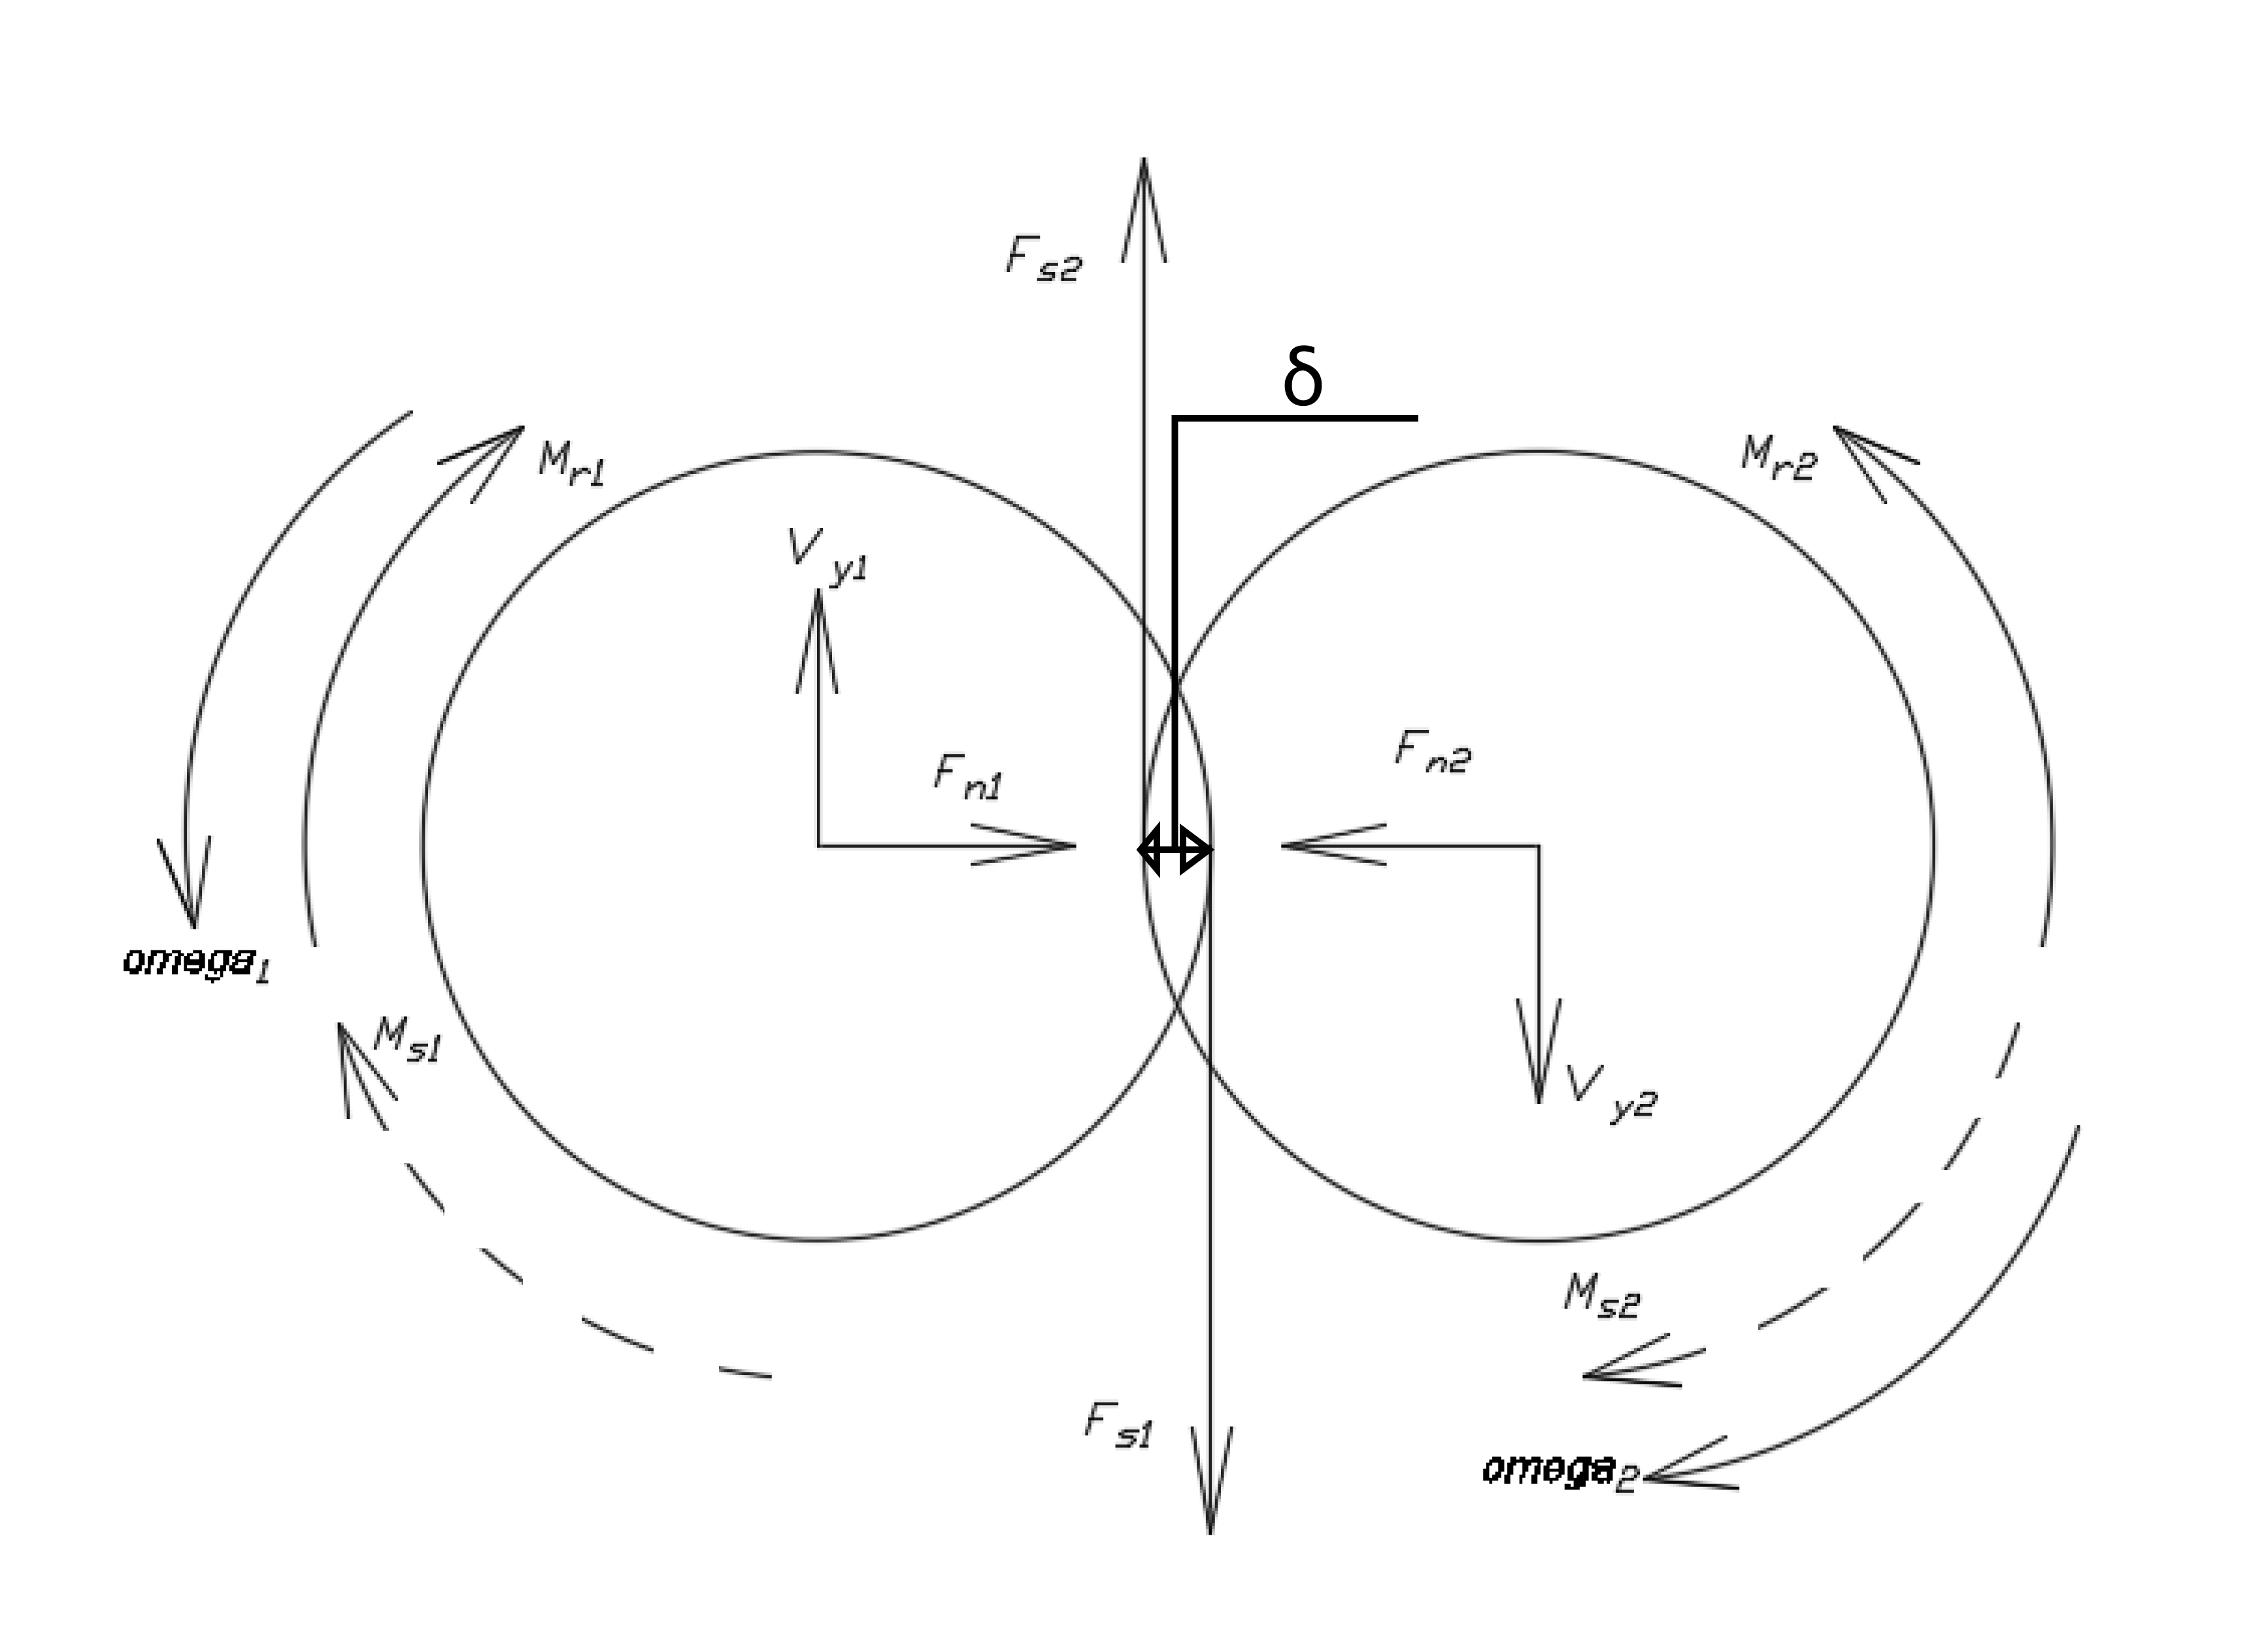
\includegraphics[width=0.8\textwidth]{sily}
	\caption{Контактные силы, возникающие в шарах при взаимодействии}
\end{figure} 
\end{frame}



















\begin{frame}
\frametitle{\insertsection} 
\framesubtitle{Контактные силы в нормальном направлении}

\begin{wrapfigure}{r}{0.15\textwidth}
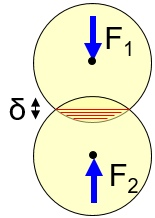
\includegraphics[width=0.15\textwidth]{vhod}
\end{wrapfigure}

\begin{equation}
\label{norm_force}
F_n = k_n \cdot \delta_n
\end{equation}

где $F_n$ --- контактная сила, возникающая в точке контакта и действующая на оба шара, [Н];

$k_n$ --- коэффициент жёсткости, [Н/м];

$\delta_n$ --- взаимное проникновение, так называемое вхождение шаров друг в друга, [м].

\begin{equation}
\label{kn_herz}
k_n = \frac{4}{3} \cdot E_{eff} \cdot \sqrt{R_{eff} \cdot \delta_n}
\end{equation}
где 
\[
\dfrac{1}{E_{eff}} = \dfrac{1 - \nu_1^2}{E_1} + \dfrac{1 - \nu_2^2}{E_2} \qquad \qquad \qquad \dfrac{1}{R_{eff}} = \dfrac{1}{R_1} + \dfrac{1}{R_2}
\]

\end{frame}

































\begin{frame}
\frametitle{\insertsection} 
\framesubtitle{Контактные силы в тангенциальном и окружном направлениях}
\begin{figure}[h!]
	\centering
	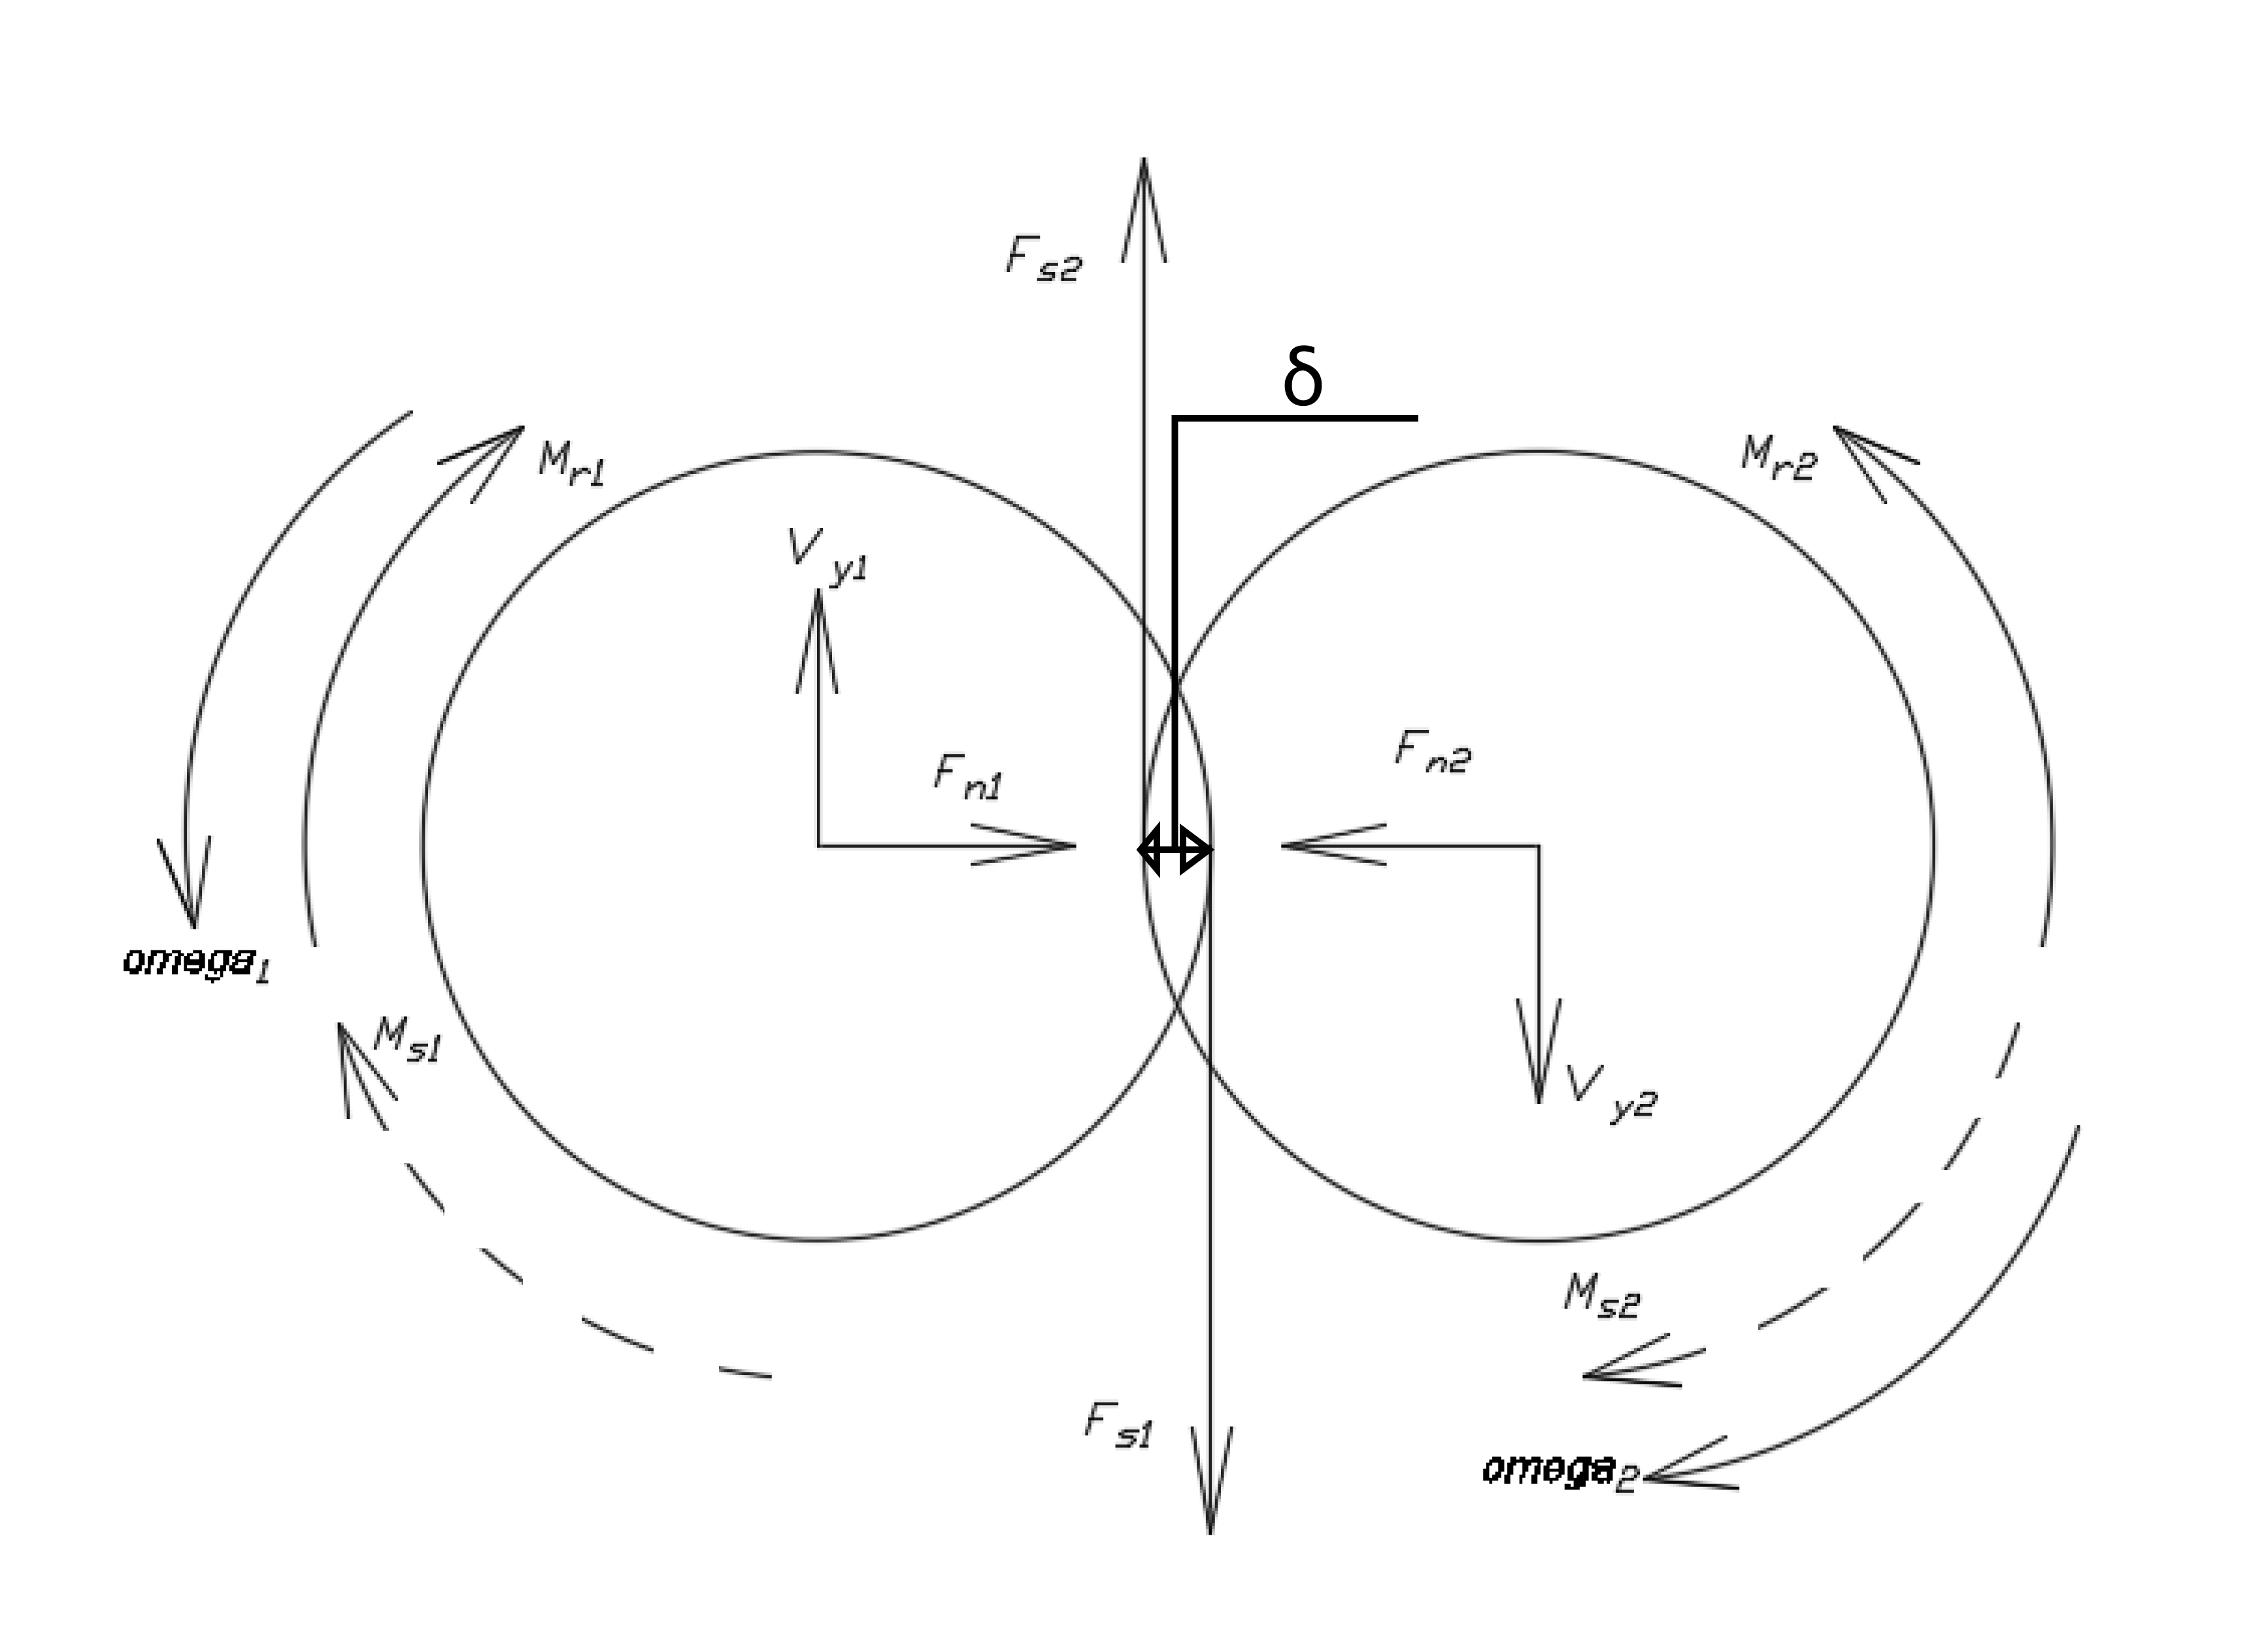
\includegraphics[width=0.55\textwidth]{sily}
\end{figure} 
\begin{align*}
F_s &= \mu_s \cdot F_n \cdot sign(v_{rel\_tan}) \qquad v_{rel\_tan} \neq 0\\
M_s &= F_s \cdot R_{eff}\\
M_r &= \mu_r \cdot F_n \cdot R_{eff} \cdot sign(\omega_{rel}) \qquad \qquad \omega_{rel} \neq 0\\
v_{rel\_tan}^{1} &= v_{y}^{1} - v_{y}^{2} - \left( \omega_1 \cdot R_1 + \omega_2 \cdot R_2 \right)\\
\omega_{rel} &= \omega_1 + \omega_2\\
\end{align*}
\end{frame}





\begin{frame}
\frametitle{\insertsection} 
\framesubtitle{Контактные силы скольжения}

\begin{figure}[h!]
	\centering
	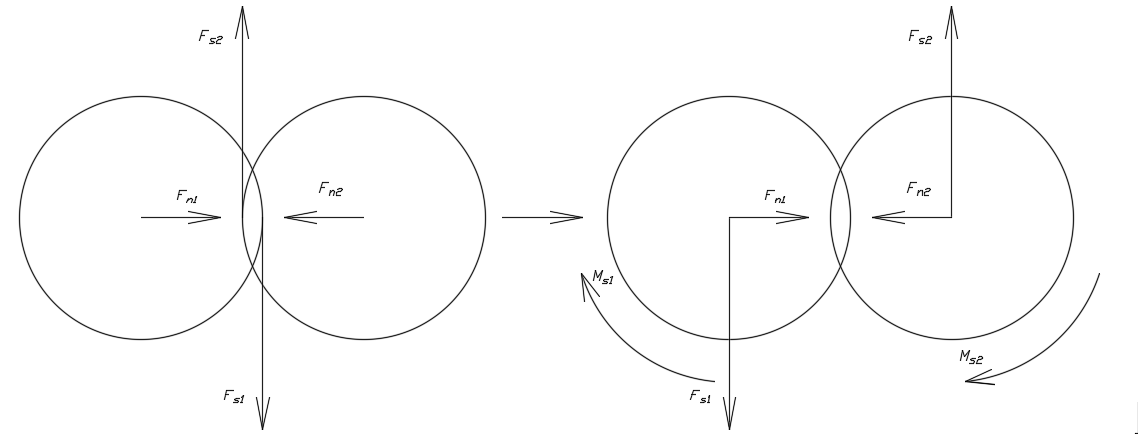
\includegraphics[width=0.8\textwidth]{fs_ms}
	\caption{Приведение силы трения скольжения к центру элемента}
	\label{pic:fs_ms}
\end{figure} 
\end{frame}






\subsection{Силы диссипации}

\begin{frame}
\frametitle{\insertsection} 
\framesubtitle{\insertsubsection}
\begin{wrapfigure}{r}{0.4\textwidth}
	\centering
	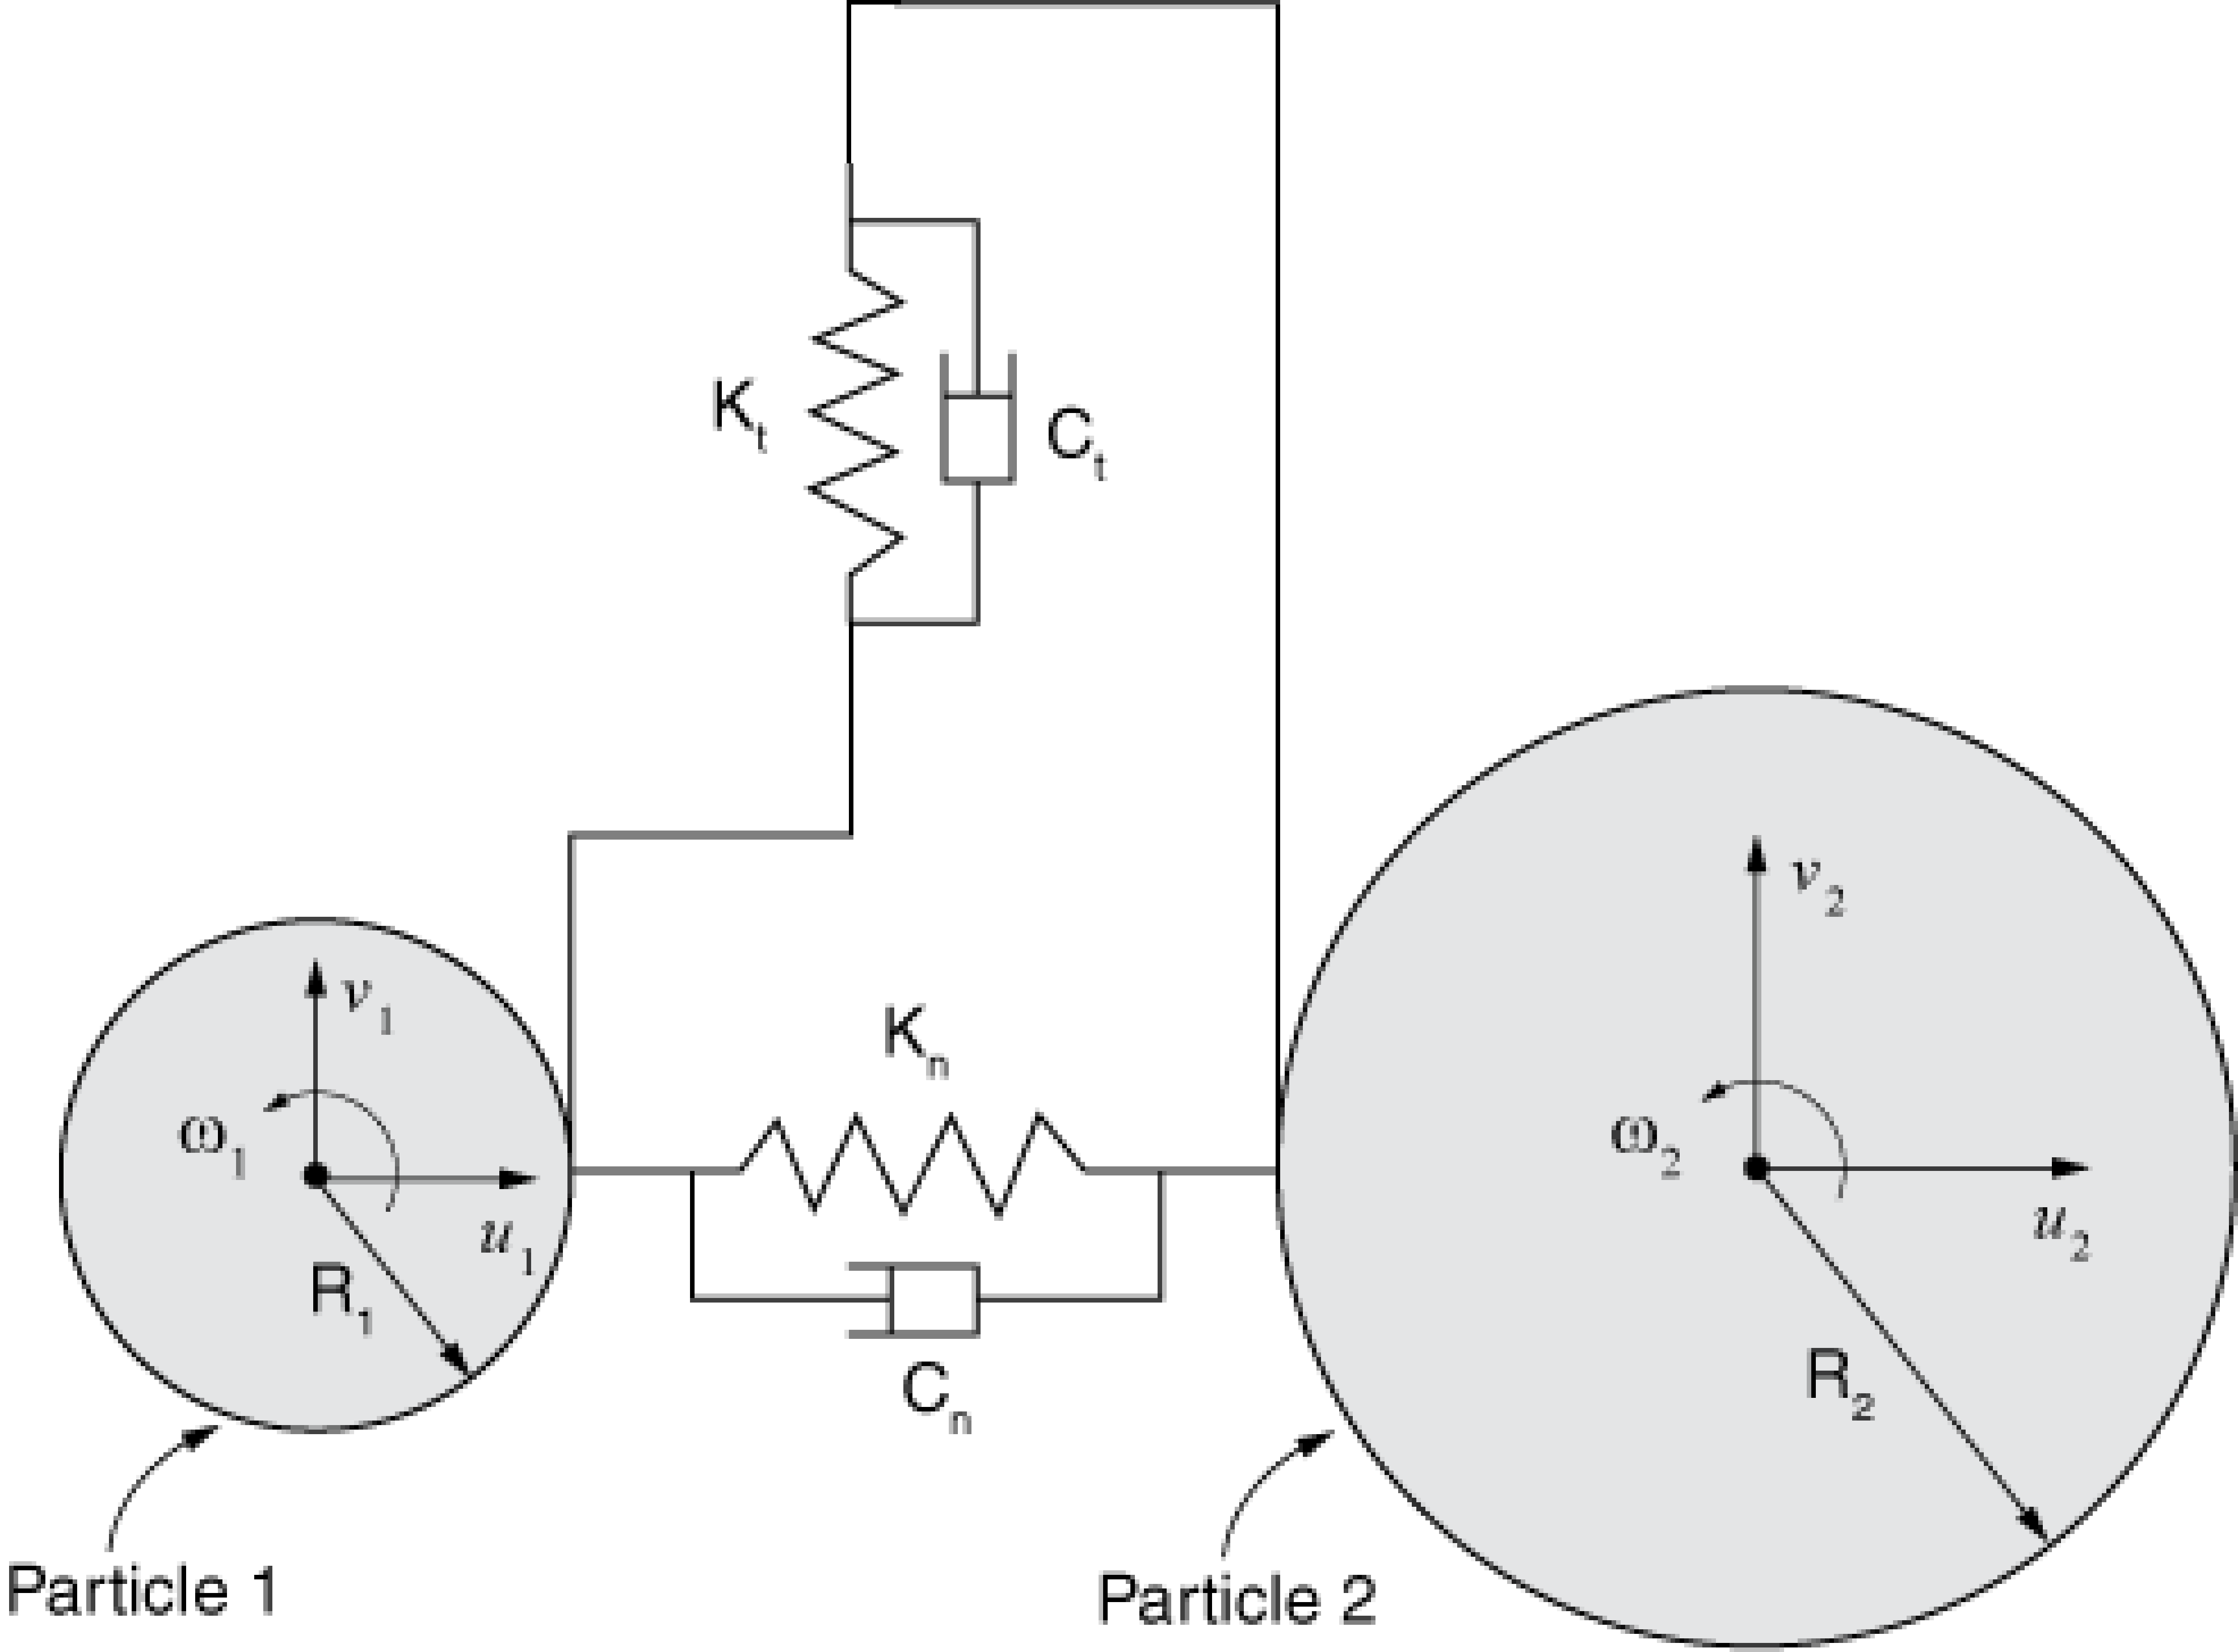
\includegraphics[width=0.4\textwidth]{dempfer}
\end{wrapfigure} 
\begin{align*}
D_n &= c_n \cdot v_{n\_rel}\\
D_t &= c_t \cdot v_{t\_rel}\\
c_n &= 2 \cdot \sqrt{m \cdot 2 \cdot E_{eff} \cdot \delta_n \sqrt{R_{eff}}} \cdot \zeta_n \\
c_t &= 4 \cdot \sqrt{m \cdot 2 \cdot G_{eff} \cdot \delta_n \sqrt{R_{eff}}} \cdot \zeta_t
\end{align*}
Караваев А. С., Копысов С. П., Сармакеева А. С. Моделирование динамики произвольных тел методом дискретных элементов //Вестник Удмуртского университета. Математика. Механика. Компьютерные науки. – 2015. – Т. 25. – №. 4. – С. 473-482.
\end{frame}














\subsection{Кинематика частиц}

\begin{frame}
\frametitle{\insertsection} 
\framesubtitle{\insertsubsection}
\begin{align}
x &= x_0 + v^x_0 \cdot \Delta t + \dfrac{a^x_0 \cdot \Delta t^2}{2} + \dfrac{b^x_0 \cdot \Delta t^3}{6}\\
y &= y_0 + v^y_0 \cdot \Delta t + \dfrac{a^y_0 \cdot \Delta t^2}{2} + \dfrac{b^y_0 \cdot \Delta t^3}{6}\\
\vartheta &= \vartheta_0 + v^{\vartheta}_0 \cdot \Delta t + \dfrac{a^{\vartheta}_0 \cdot \Delta t^2}{2} + \dfrac{b^{\vartheta}_0 \cdot \Delta t^3}{6}
\end{align}
\begin{align}
b_n &= \dfrac{a_{t + \Delta t} - a_{t}}{\Delta t} \\
b_t &= \dfrac{a_{t + \Delta t} - a_{t}}{\Delta t} \\
b_{\vartheta} &= \dfrac{\varepsilon_{t + \Delta t} - \varepsilon_{t}}{\Delta t} 
\end{align}

\[
\left\lbrace b \right\rbrace^{glob} = [T] \cdot \left\lbrace b \right\rbrace^{loc}
\]
\end{frame}










\begin{frame}
\frametitle{\insertsection} 
\framesubtitle{Блок-схема итерационного уточнения}

\begin{figure}[H]
	\centering
	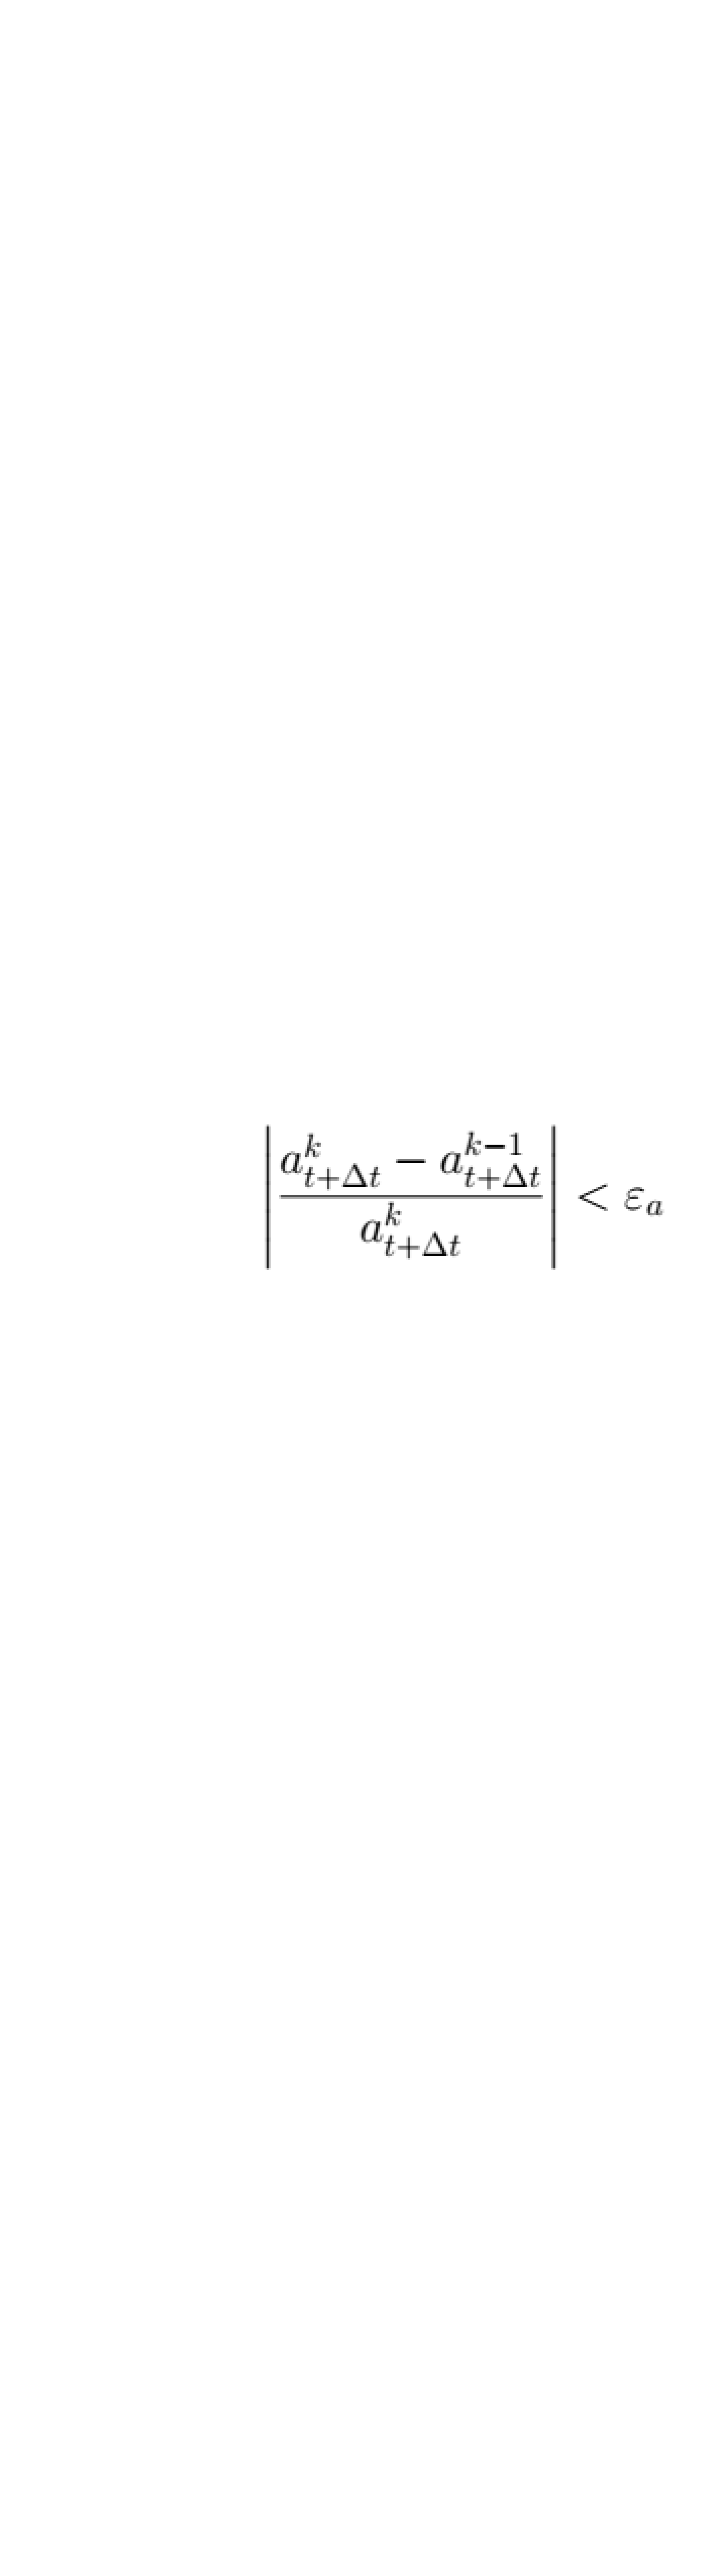
\includegraphics[width=0.2\textwidth]{kriter_big}
	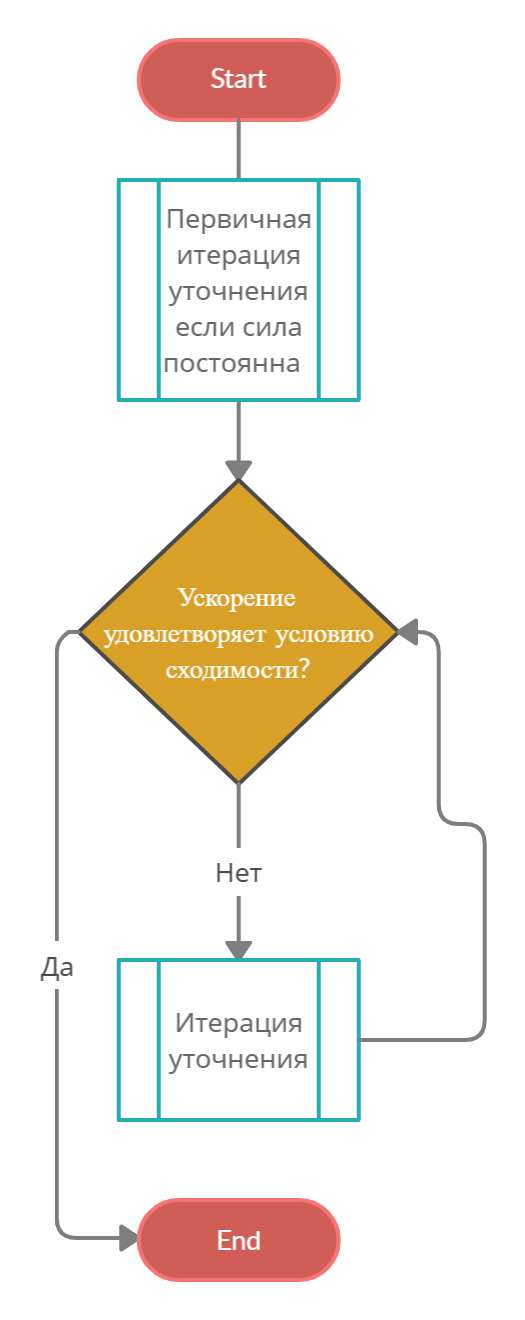
\includegraphics[width=0.3\textwidth]{iter_cicle} 
	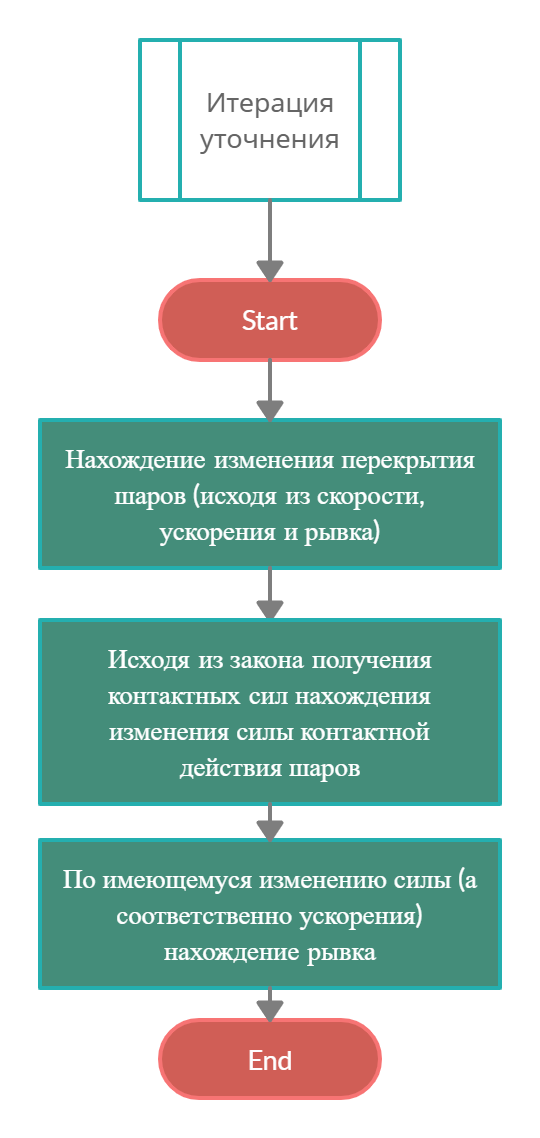
\includegraphics[width=0.3\textwidth]{iter_one}
	\label{pic:iter}
\end{figure} 

\end{frame}












\begin{frame}
\frametitle{\insertsection} 
\framesubtitle{Совокупность уравнений}
\alt<2> {
\[
\left\lbrace
\begin{aligned}
\overline{m \cdot a_t} &= \overline{G}\\
\overline{I \cdot \varepsilon_t} &= 0\\
\overline{v}_{t} &= \overline{v}_{t - \Delta t} + \overline{a}_t \cdot \Delta t \\
\overline{s}_{t} &= \overline{s}_{t - \Delta t} + \overline{v}_{t - \Delta t} \cdot \Delta t + \dfrac{\overline{a}_t \cdot \Delta t^2}{2} \\
v_{t}^{\vartheta} &= v^{\vartheta}_{t - \Delta t}  \\
\vartheta_{t} &= \vartheta_{t - \Delta t} + v^{\vartheta}_{t - \Delta t} \cdot \Delta t
\end{aligned}
\right.
\]
} 
{
\[
\left\lbrace
\begin{aligned}
\overline{m \cdot a_t} &= \overline{F_n} + \overline{F_s} + \overline{D} + \overline{G}\\
\overline{I \cdot \varepsilon_t} &= \overline{M_s} + \overline{M_r}\\
\overline{v}_{t} &= \overline{v}_{t - \Delta t} + \overline{a}_t \cdot \Delta t + \dfrac{\overline{b}_t \cdot \Delta t^2}{2} \\
\overline{s}_{t} &= \overline{s}_{t - \Delta t} + \overline{v}_{t - \Delta t} \cdot \Delta t + \dfrac{\overline{a}_t \cdot \Delta t^2}{2} +  \dfrac{\overline{b}_t \cdot \Delta t^3}{6}\\
v_{t}^{\vartheta} &= v^{\vartheta}_{t - \Delta t} + \varepsilon_t \cdot \Delta t\\
\vartheta_{t} &= \vartheta_{t - \Delta t} + v^{\vartheta}_{t - \Delta t} \cdot \Delta t + \dfrac{\varepsilon_t \cdot \Delta t^2}{2} + \dfrac{b^{\vartheta}_t \cdot \Delta t^3}{6} 
\end{aligned}
\right.
\]
}


\end{frame}
























\section{Результаты работы}

\begin{frame}
\frametitle{\insertsection} 
\framesubtitle{Постановка задачи}

\begin{center}
\begin{tabular}{|c|c|}
\hline
Модуль продольной упругости & 2$\times 10^{11}$ Па  \\ 
\hline
Модуль сдвига & 8$\times 10^{10}$ Па \\  
\hline
Плотность материала & 7800 кг/м$^3$ \\
\hline
К-т диссипации в норм-ом направлении & 0.1 \\
\hline
К-т диссипации в танген-ом направлении & 0.1 \\
\hline
К-т трения скольжения & 0.1 \\
\hline
К-т трения качения & 0.05 \\
\hline
Радиус шаровой мельницы & 2.5 м \\
\hline
Радиус шаров & 0.1 м \\
\hline
Количество шаров & 120 \\
\hline
Процент заполненности мельницы & 21 \% \\
\hline
Шаг по времени & 10$^{-5}$ сек \\
\hline
\end{tabular}
\end{center}

\end{frame}

\subsection{Каскадный режим}

\begin{frame}
\frametitle{\insertsection} 
\framesubtitle{\insertsubsection}
	\begin{figure}[ht]
 		\includemovie[
 			poster,
     		externalviewer,
     		inline=false,
     		text={\small Каскадный режим работы шаровой мельницы (2 об/мин)}]{}{}
     		{kaskad_result.mp4}
\end{figure}
	\alt<2> {
	\begin{figure}[H]
	\centering
	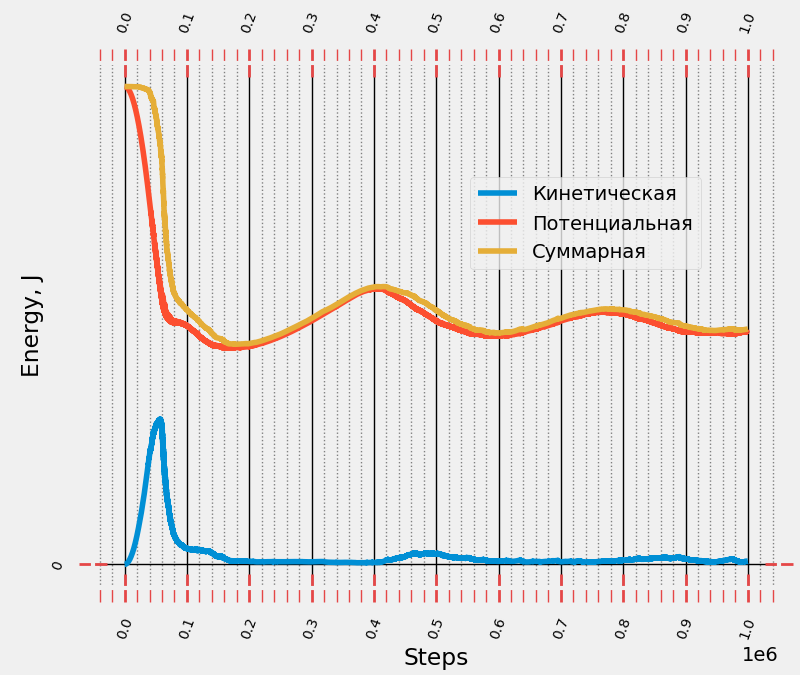
\includegraphics[width=0.5\textwidth]{kaskad_energy}
	\caption{График изменения энергии во времени при каскадном режиме работы мельницы}
	\label{pic:kaskad_energy}
\end{figure} 
}
{
\begin{figure}[H]
	\centering
	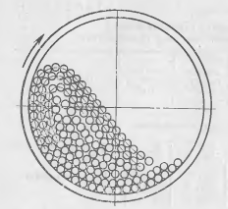
\includegraphics[width=0.5\textwidth]{kaskad_theory} 
	\caption{Теоретическая картина каскадного режима}
\end{figure}
}
\end{frame}










\subsection{Смешанный режим}

\begin{frame}
\frametitle{\insertsection} 
\framesubtitle{\insertsubsection}

\begin{figure}[ht]
 		\includemovie[
 			poster,
     		externalviewer,
     		inline=false,
     		text={\small Смешанный каскадно-водопадный режим работы (14 об/мин)}]{}{}
     		{smeshan_result.mp4}
\end{figure}

\alt<2> {
\begin{figure}[H]
	\centering
	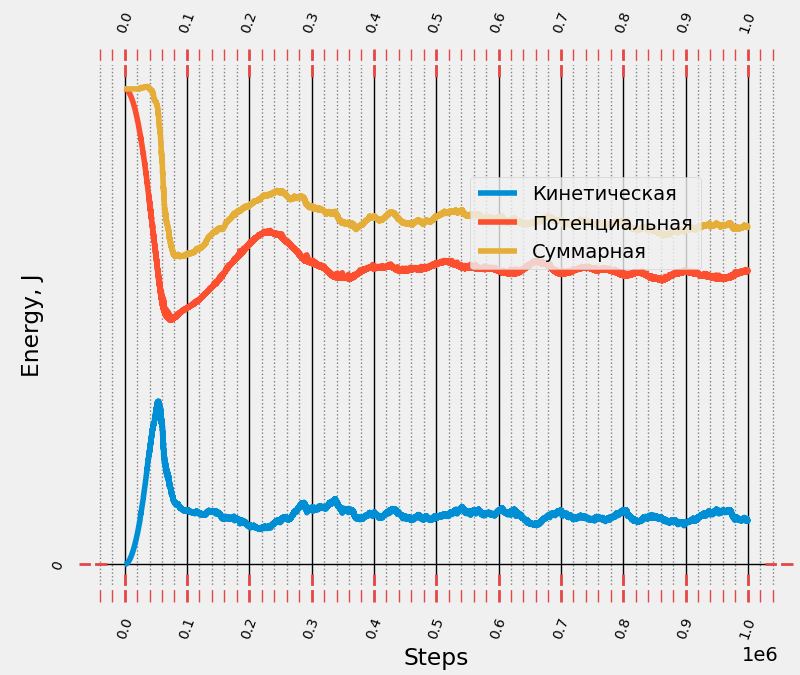
\includegraphics[width=0.5\textwidth]{smeshan_energy} 
	\caption{График изменения энергии во времени при смешанном каскадно-водопадном режиме работы мельницы}
	\label{pic:smeshan_energy}
\end{figure} 
}
{
\begin{figure}[H]
	\centering
	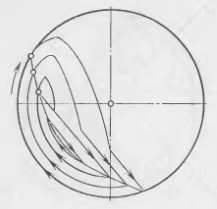
\includegraphics[width=0.5\textwidth]{smeshan_theory} 
	\caption{Теоретическая картина смешанного режима}
\end{figure}
}
\end{frame}





\subsection{Водопадный режим}

\begin{frame}
\frametitle{\insertsection} 
\framesubtitle{\insertsubsection}

\begin{figure}[ht]
 		\includemovie[
 			poster,
     		externalviewer,
     		inline=false,
     		text={\small Водопадный режим работы шаровой мельницы (17 об/мин)}]{}{}
     		{vodopad_result.mp4}
\end{figure}
\alt<2> {
\begin{figure}[H]
	\centering
	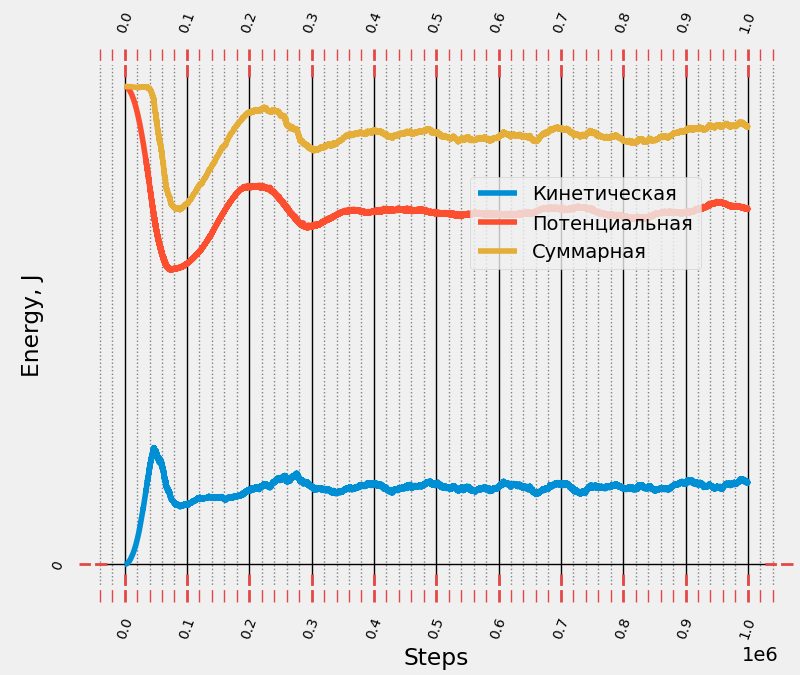
\includegraphics[width=0.5\textwidth]{vodopad_energy} 
	\caption{График изменения энергии во времени при водопадном режиме работы мельницы}
	\label{pic:vodopad_energy}
\end{figure} 
}
{
\begin{figure}[H]
	\centering
	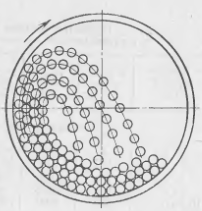
\includegraphics[width=0.5\textwidth]{vodopad_theory} 
	\caption{Теоретическая картина водопадного режима}
\end{figure}
}

\end{frame}









\subsection{С превышением критической частоты}

\begin{frame}
\frametitle{\insertsection} 
\framesubtitle{\insertsubsection}
\begin{figure}[ht]
 		\includemovie[
 			poster,
     		externalviewer,
     		inline=false,
     		text={\small Превышение критической частоты (30 об/мин)}]{}{}
     		{kritic_result.mp4}
\end{figure}
\alt<2> {
\begin{figure}[H]
	\centering
	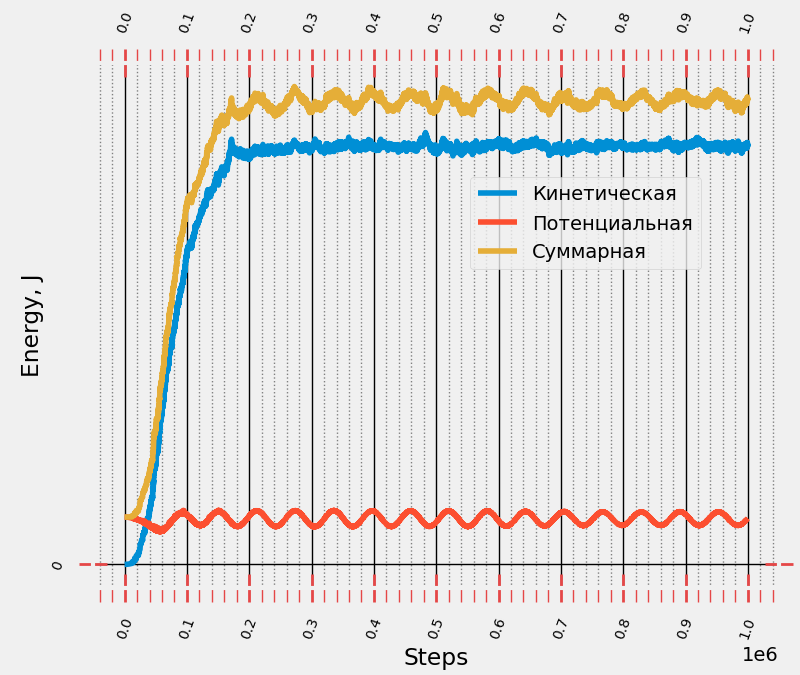
\includegraphics[width=0.5\textwidth]{kritic_energy} 
	\caption{График изменения энергии во времени при превышении критической частоты}
\end{figure}
}
{
\begin{figure}[H]
	\centering
	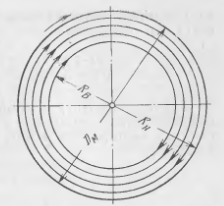
\includegraphics[width=0.5\textwidth]{kritic_theory} 
	\caption{Теоретическая картина закритического режима}
\end{figure}
}
\end{frame}


\begin{frame}
\centering
Спасибо за внимание!
\end{frame}

\section{Доп. материалы}

\begin{frame}
\frametitle{\insertsection} 
\framesubtitle{Шар-стенка}

\begin{figure}[h!]
	\centering
	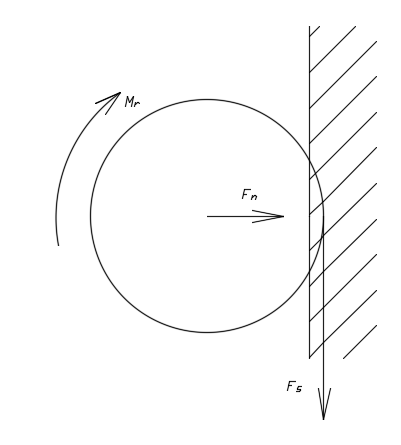
\includegraphics[width=0.5\textwidth]{ball_wall}
\end{figure} 
\end{frame}


\begin{frame}
\frametitle{\insertsection} 
\framesubtitle{Упрощения МДЭ}

\begin{figure}[h!]
	\centering
	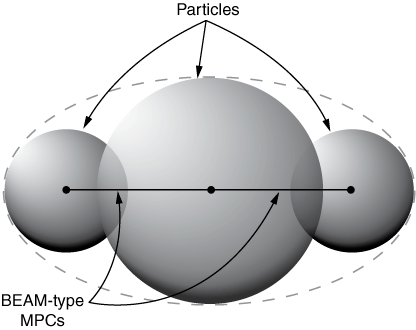
\includegraphics[width=0.7\textwidth]{dem-rigid-cluster}
\end{figure} 
\end{frame}




 \end{document}
